\section{\normalsize Эффект Джоуля--Томсона (дифференциальный и интегральный). Температура инверсии.} 
\paragraph{Дифференциальный эффект Джоуля--Томпсона.} Рассмотрим процесс Джоуля--Томпсона: адиабатическое стационарное течение газа через пористую перегородку, под действием разности давлений

\begin{wrapfigure}{L}{7cm}
	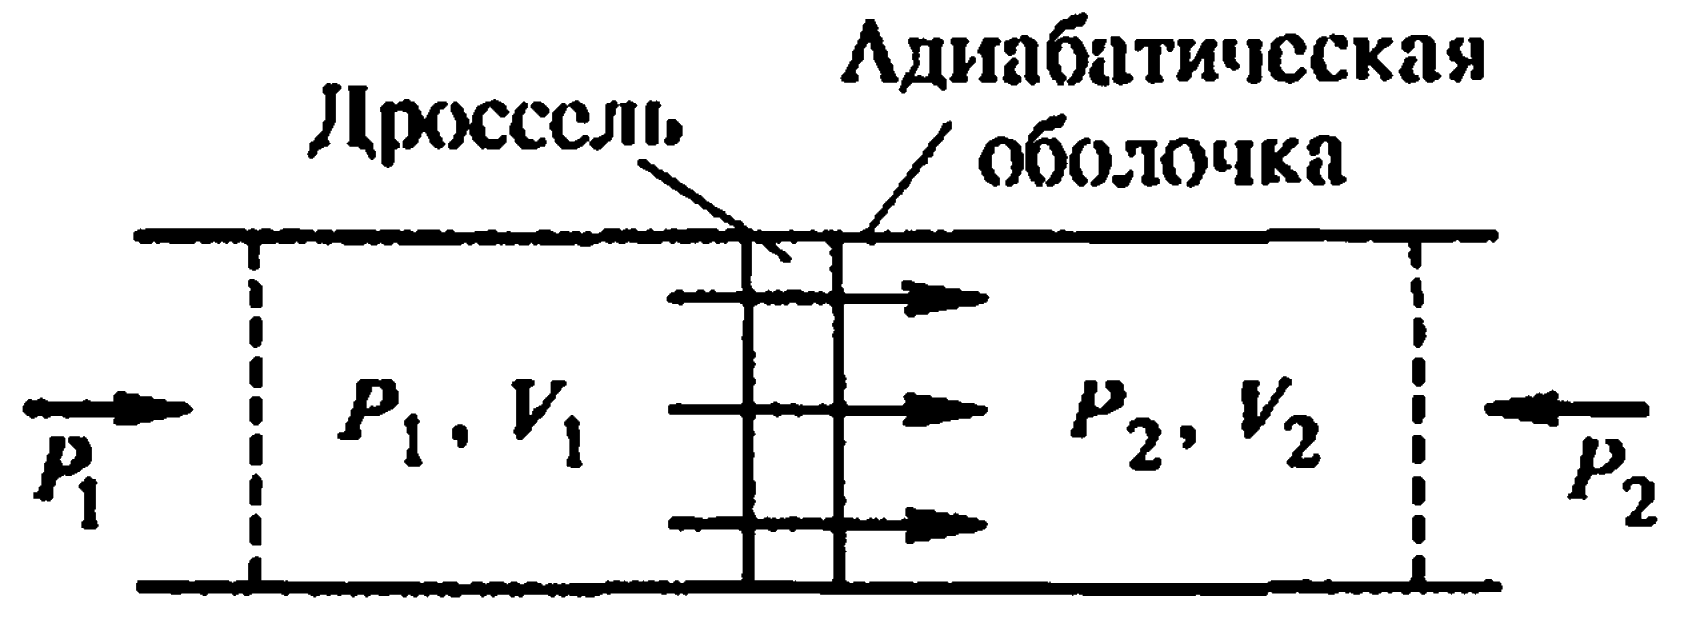
\includegraphics[width=70mm]{ris22_1.png}
\end{wrapfigure}
 по разные стороны от пробки. Изменение температуры в этом процессе --- \textbf{эффект Джоуля-Томпсона}. Течение медленное, следовательно можно пренебречь кинетической энергией. Тогда по первому началу термодинамики $Q=0\Rightarrow\\0=\Delta U+A=U_2-U_1+P_2V_2-P_1V_1=I_2-I_1\Leftrightarrow I_1=I_2$. В процессе Джоуля--Томпсона $I=const$.\\
 Пусть теперь по разные стороны от перегородки разность давлений мала. Найдем $\Delta T:$ $$\Delta I = \chpr{I}{T}{P}\Delta T+\chpr{I}{P}{T}\Delta P=0\Rightarrow\chpr{I}{T}{P}=C_P,\ \chpr{I}{P}{T}=V-T\chpr{V}{T}{P}\Rightarrow$$
 $$\Rightarrow\left(\dfrac{\Delta T}{\Delta P}\right)_I=\dfrac{T\Chpr{V}{T}{P}-V}{C_P}$$
 Если газ идеальный, то $V=\dfrac{RT}{P},\ T\chpr{V}{T}{P}=V\Rightarrow\Delta T=0$, то есть для идеальных газов эффекто Джоуля--Томпсона не имеет места. Повышение или понижение температуры реального газа при протекании через пробку при малых $\Delta T$ и $\Delta P$ $\left(\text{для замены их отношения на } \Chpr{T}{P}{I}\right)$ называется \textbf{дифференциальным эффектом Джоуля--Томпсона}.\\
 Так как течение происходит от большего давления к меньшему, то $\Delta P<0$, значит если $\frac{\Delta T}{\Delta P}>0$, то эффекто Джоуля--Томпсона \textbf{положительный}, а если соответственно $\frac{\Delta T}{\Delta P}<0$ --- \textbf{отрицательный}.
 
 \begin{wrapfigure}{R}{4cm}
 	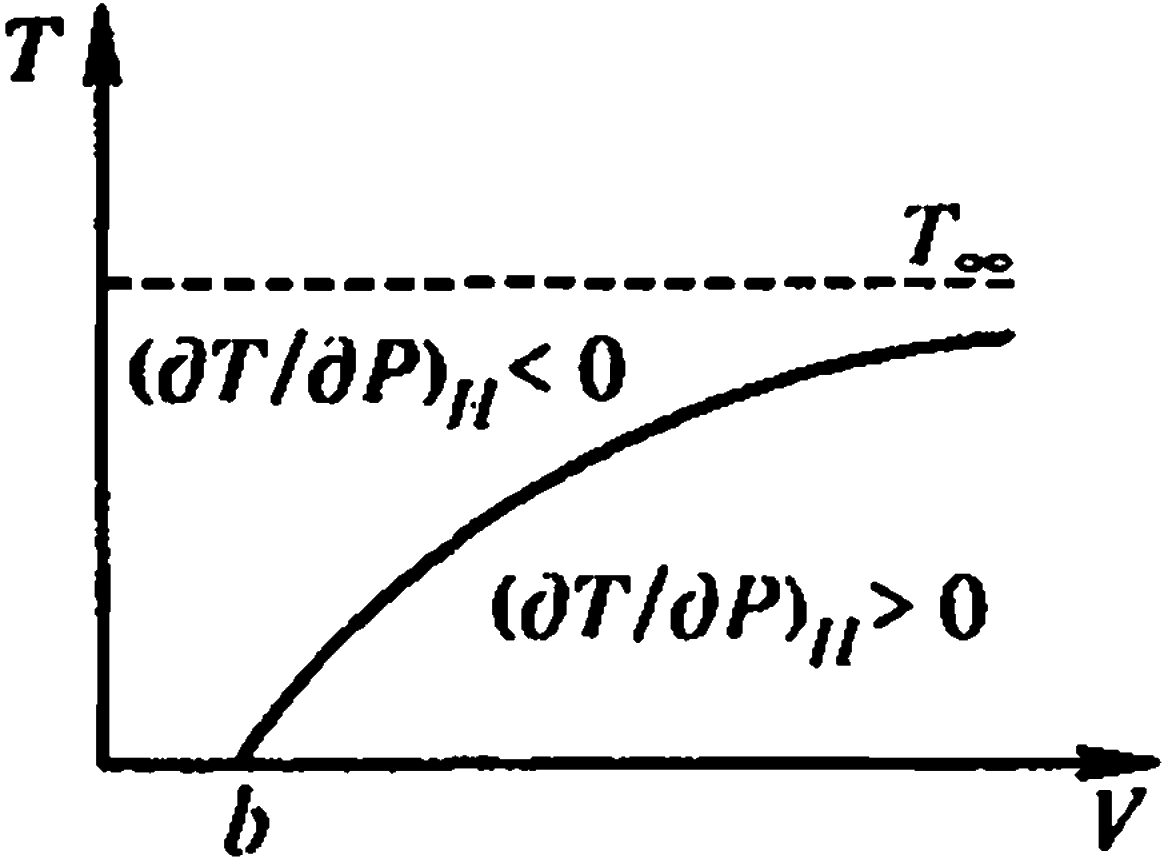
\includegraphics[width=40mm]{ris22_2.png}
 \end{wrapfigure}
 Вычисляя $\chpr{V}{T}{P}=\dfrac{-\Chpr{P}{T}{V}}{\Chpr{P}{V}{T}}$ из уравнения Ван-дер-Ваальса получаем:
 $$\dfrac{\Delta T}{\Delta P}=-\dfrac{T\Chpr{P}{T}{V}+V\Chpr{P}{V}{T}}{C_P\Chpr{P}{V}{T}}=\dfrac{\frac{bRT}{(V-b)^2}-\frac{2a}{V^2}}{C_P\Chpr{P}{V}{T}}$$
 \paragraph{Температура инверсии.} Пояснение к графику: $T_\infty\equiv T_i,\ H\equiv I$. В случае разреженного газа можно отбросить малые поправки $a$ и $b$ высших порядков $\Rightarrow\dfrac{\Delta T}{\Delta P}=\dfrac{\frac{2a}{RT}-b}{C_P}$. При $T_i=\dfrac{2a}{RB}=\dfrac{27}{4}T_\text{кр.}$ --- температуре инверсии дифференциального эффекта Джоуля--Томпсона  $\Delta T=0$. Газ ниже этой температуры охлаждается, выше --- нагревается в процессе Джоуля--Томпсона. \\
 \paragraph{Интегральный эффект Джоуля--Томпсона.} Пусть теперь по разные стороны от перегородки $\Delta P$ велика, тогда велика и $\Delta T$. Тогда мы имее дело с \textbf{интегральным законом Джоуля--Томпсона.}
 \begin{equation}
 T_2-T_1=\int_{P_1}^{P_2}\chpr{T}{P}{I}dP=\int_{P_1}^{P_2}\dfrac{T\Chpr{V}{T}{P}-V}{C_P}dP
 \label{ur22}
 \end{equation}
Если во всем диапазоне давлений дифференциального эффекта Джоуля--Томпсона положительный, то и интегральный будет положительным. Масимальное охлаждение из начального состояния $T_1,\ P_1$: 
$$\dfrac{d}{dP_1}(T_2-T_1)=\dfrac{dT_2}{dP_1}=-\chpr{T}{P}{I}=0\text{ --- условие максимума записанное при }P=P_1,\ T=T_1$$
Но $\chpr{T}{P}{I}=0$ --- уравнение кривой инверсии дифференциального эффекта Джоуля--Томпсона, следовательно, для максимального охлаждения  \textbf{???} на кривой инверсии.\\
Формула (\ref{ur22}) интегрируется до конца в случае, когда в начальном состоянии газ под высоким давлением, а после прохода через вентиль его можно рассматривать как идеальный.
$$I_1=I_2\Leftrightarrow\int_{T_0}^{T_1}C_vTdT-\dfrac{a}{V_1}+P_1V_1=\int_{T_0}^{T_2}C_VTdT-\dfrac{a}{V_2}+P_2V_2\ \underset{\tfrac{a}{V_2}\rightarrow0}{\longrightarrow}\int_{T_2}^{T_1}C_VTdT-\dfrac{a}{V_1}+P_1V_1=RT_2$$
$$\overline{C_V}(T_1-T_2)-\dfrac{2a}{V_1}+\dfrac{RT_1V_1}{V_1-b}=RT_2,$$
где $\overline{C_V}$ --- средняя теплоемкость при $V=const$ в диапазоне $T_1\leftrightarrow T_2$. В итоге получим:


\begin{wrapfigure}{R}{52mm}
	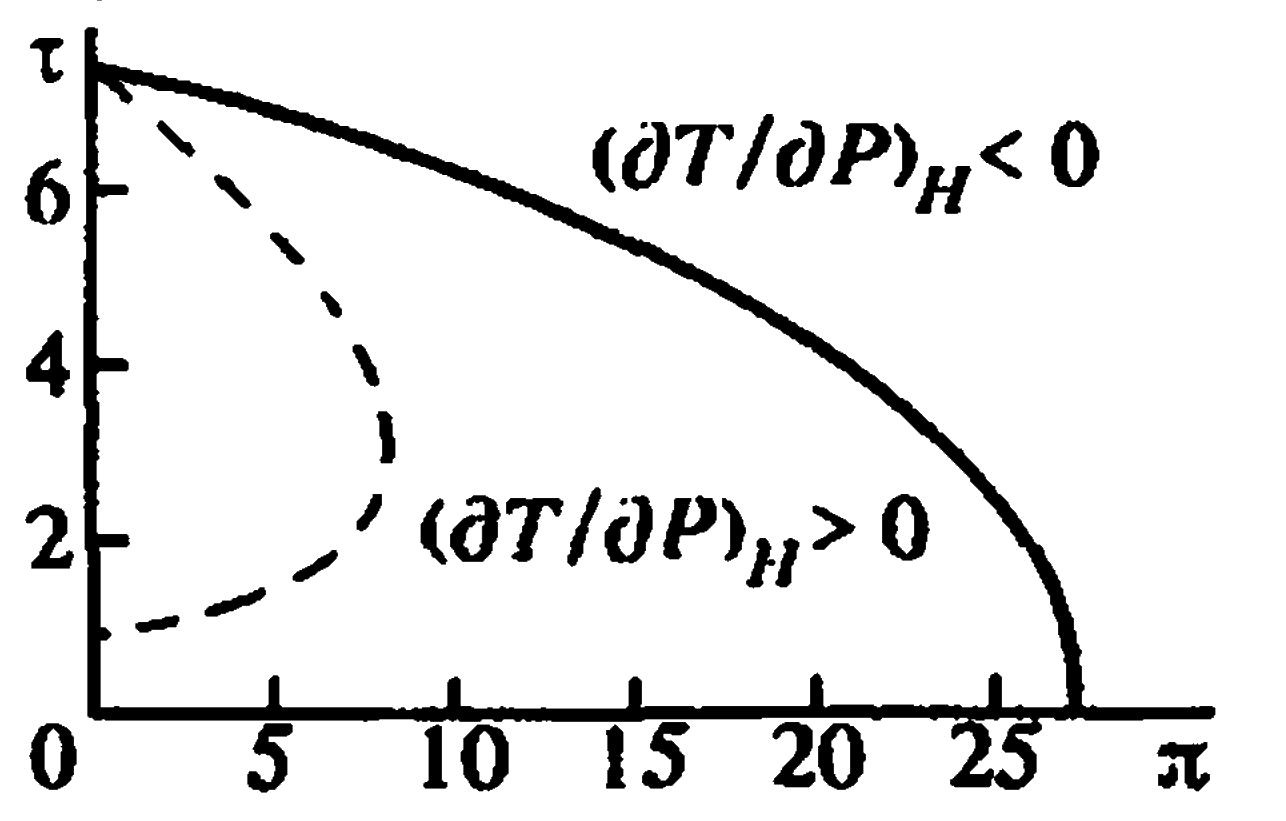
\includegraphics[width=50mm]{ris22_3.png}
	\caption{штрих. линия - кривая инверсии диф. эффекта}
\end{wrapfigure}
$$T_2-T_1=\dfrac{1}{R+\overline{C_V}}\left(\dfrac{RbT_1}{V_1-b}-\dfrac{2a}{V_1}\right)$$
Так как знаменатель положительный, то знак эффекта определяется знаком числителя.
\begin{enumerate}
	\item $T_1<\dfrac{2a}{Rb}\dfrac{V_1-b}{V_1}$ --- эффект положительный (охлаждение)
	\item $T_1>\dfrac{2a}{Rb}\dfrac{V_1-b}{V_1}$ --- эффект отрецательный (нагревание)
	\item $T_1=\dfrac{2a}{Rb}\dfrac{V_1-b}{V_1}$ --- температура инверсии интегрального эффекта Джоуля--Томпсона
\end{enumerate}
$\tau=27/4\dfrac{\varphi-1/3}{\varphi}$ --- в приведенном виде, $\pi=27-16/27\tau^2\Leftrightarrow\tau=3/4\sqrt{81-3\pi}$